\chapter{Teorema de Separación}

En esta sección introducimos algunos resultados sobre separación. En general, estos nos aportan herramientas para poder concluir cuándo dos subconjuntos convexos pueden ser separados mediante un hiperplano. En la siguiente imagen vemos un ejemplo sobre la situación en la que nos encontramos:

\begin{figure}[h!]
\begin{center}
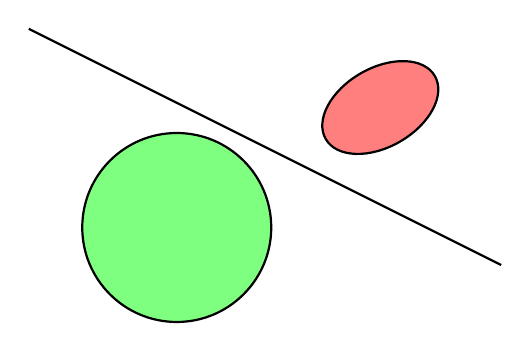
\begin{tikzpicture}[thick,fill opacity=0.5]
\filldraw[fill=red][rotate = 30] (0:4cm) ellipse (8mm and 5 mm);
\filldraw[fill=green] (1cm:1cm) circle (12mm);
\draw (-1,3) -- (5,0);
%\node at (0.9cm,0.6cm) {\large A};
%\node at (3.5cm,2.1cm) {\large B};
\end{tikzpicture}
\end{center}
\caption{Situación de teoremas de separación}
\end{figure}

Expones un resultado sencillo en el que solo involucramos un conjunto

\begin{teoremaBox}\label{sep1}
Dado $ N \in \NN $ y sea $ C \subset \RR^N $ convexo y definimos
\[
\delta := \inf\{ \norm{c}: c \in C \}.
\]
Entonces, existe $ x_0 \in \RR^N $ tal que si $ c \in C $ se cumple que $ \delta \leq \langle x_0,c\rangle $.
\end{teoremaBox}
\begin{proof}
En primer lugar, vamos a reescribir la tesis del teorema. Queremos ver que:
\[
\exists x_0 \in \RR^N : c \in C \Longrightarrow \delta \leq \langle x_0,c\rangle.
\]
\[
\big\Updownarrow
\]
\[
\exists \alpha > 0, \exists x_0 \in \alpha B_{\RR^N} : c \in C \Longrightarrow \delta \leq \langle x_0,c\rangle.
\]
\[
\big\Updownarrow
\]
\[
\exists \alpha > 0, \exists x_0 \in \alpha B_{\RR^N} : \delta \leq \inf_{c\in C}\langle x_0,c\rangle.
\]
\[
\big\Updownarrow
\]
\[
\exists \alpha > 0 : \delta \leq \max_{x\in \alpha B_{\RR^N}}\inf_{c\in C}\langle x,c\rangle.
\]
Llamamos $ \topSpace := \alpha B_{\RR^N}$ que es compacto y conexo, $ \topSpaceY:= C$ convexo y $ f $ función a la real y continua con valores en $ \topSpace \times \topSpaceY $ definida como $ f(x,y):=\langle x,y \rangle $ (al ser $ f $ continua, en particular es superiormente semicontinua). Aplicamos el teorema Minimax, teorema (\ref{MinMax}), y obtenemos que probar la última desigualdad es equivalente a probar que
\[
\exists \alpha > 0 : \delta \leq \inf_{c\in C}\max_{x\in \alpha B_{\RR^N}}\langle x_0,c\rangle.
\]
Tenemos que $ \max_{x\in \alpha B_{\RR^N}}\langle x,c\rangle \leq \alpha \norm{c} $ por la desigualdad de Cauchy–Schwarz. Así, debemos demostrar que
\[
\exists \alpha > 0 : \delta \leq \inf_{c\in C} \alpha \norm{c} \leq \alpha  \inf_{c\in C}\norm{c} = \alpha \delta.
\]
Pero esta desigualdad es cierta tomando, por ejemplo, $ \alpha = 1 $.
\end{proof}

Ahora, vamos a hacer una generalización de este resultado.
\begin{teoremaBox}\label{separacion1}
Sean $ A,B $ subconjuntos convexos de $ \RR^N $ para $ N \in \NN $ tal que $ A $ es cerrado, $ B $ es compacto y $ A \cap B = \emptyset$. Entonces existe $ x_0 \in \RR^N $ tal que
\[
\sup_{a \in A} \langle x_0,a\rangle < \inf_{b\in B} \langle x_0,b\rangle.
\]
\end{teoremaBox}
\begin{proof}
En primer lugar, veamos que $ \dist(A,B) > 0 $ donde la distancia viene dada por $\dist(A,B) = \inf\{ \norm{a-b} : a\in A, b\in B\}$. Para ello, razonemos por reducción al absurdo. Suponemos $ \dist(A,B) = 0 $, entonces existe una sucesión $ \{u_n\}_{n\in\NN} \subset A-B $ tal que $ \{u_n\}_{n\in\NN} \longrightarrow 0 $. Para $ n\in\NN $ tenemos que $ u_n = a_n - b_n $ con $ a_n \in A $ y $ b_n \in B $. De este modo obtenemos las sucesiones $ \{a_n\}_{n\in\NN} \subset A $ y $ \{b_n\}_{n\in\NN} \subset B $. Como $ B $ es compacto, existe una sucesión parcial convergente, es decir, existe $ \sigma: \NN \longrightarrow \NN $ estrictamente creciente tal que $ \{b_{\sigma(n)}\}_{n\in\NN} \longrightarrow b$ con $ b \in B $. Así,
\[
\norm{a_{\sigma(n)}-b} = \norm{a_{\sigma(n)} - b_{\sigma(n)} + b_{\sigma(n)} - b} \leq  \norm{a_{\sigma(n)} - b_{\sigma(n)}} + \norm{b_{\sigma(n)} - b}.
\]
Entonces tenemos que $ \norm{a_{\sigma(n)}-b} \longrightarrow 0 $ ya que $ \{b_{\sigma(n)}\}_{n\in\NN} \longrightarrow b$ y como $ \norm{a_n - b_n}\longrightarrow 0$ también se cumple que $ \norm{a_{\sigma(n)} - b_{\sigma(n)}}\longrightarrow 0$. Llegamos a que $ \{a_{\sigma(n)}\}_{n\in\NN} \longrightarrow b$. Al ser $ A $ cerrado se debe cumplir que $ b \in A $ lo cual es imposible ya que $ A \cap B = \emptyset$. \\

Ahora, aplicamos el teorema (\ref{sep1}) a $ C:= B-A $. Notar que $ C $ es convexo por serlo $ A $ y $ B $. Obtenemos entonces que existe $ x_0 \in \RR^N $ tal que si $ c \in C $ se cumple que:
\[
\delta = \inf_{c \in C} \norm{c} \leq \langle x_0, c\rangle.
\]
Por la definición de $ C $, se tiene que:
\[
\delta = \inf\{ \norm{b-a} : a\in A, b\in B\} = \dist(A,B) > 0.
\] 
Del mismo modo, $ c = b-a $ para todo $ c \in C $ con $ a \in A $ y $ b \in B $. Así.
\[
\exists x_0 \in \RR^N: a\in A, b\in B \Longrightarrow 0 <\delta \leq \langle x_0, b-a\rangle = \langle x_0, b\rangle - \langle x_0,a\rangle.
\]
\[
\big\Updownarrow
\]
\[
\exists x_0 \in \RR^N: a\in A, b\in B \Longrightarrow \langle x_0, a\rangle + \delta \leq \langle x_0, b\rangle ,\text{ con } \delta > 0.
\]
\[
\big\Updownarrow
\]
\[
\exists x_0 \in \RR^N \Longrightarrow \sup_{a\in A}\langle x_0, a\rangle + \delta \leq \inf_{b \in B}\langle x_0, a\rangle, \text{ con } \delta > 0.
\]
\[
\big\Updownarrow
\]
\[
\exists x_0 \in \RR^N : \sup_{a\in A}\langle x_0, a\rangle < \inf_{b \in B}\langle x_0, a\rangle.
\]
Por ello, queda probado el teorema.
\end{proof}

El teorema de separación anterior podemos escribirlo no solo en $ \RR^N $ sino que se puede generalizar a cualquier espacio normado finito dimensional. A continuación, exponemos otro teorema de separación válido solo en espacios normados reales pero que con unas hipótesis más débiles podemos obtener una tesis parecida.

\begin{teoremaBox}
Sea $ N \in \NN $ y $ A \text{ y } B$ dos subconjuntos convexos y disjuntos de $ \RR^N $. Entonces existe $ x_0 \in \RR^N \setminus \{0\} $ tal que
\[
\sup_{a \in A} \langle x_0,a\rangle \leq \inf_{b\in B} \langle x_0,b\rangle.
\]
\end{teoremaBox}
\begin{proof}
Al igual que en el teorema anterior, podemos reducir la prueba al caso en que $ C $ es un subconjunto de $ \RR^N $ convexo de forma que $ 0 \notin C $, demostrando que:
\[
\exists x_0 \in \RR^N \setminus \{0\}: \quad \sup_{c \in C} \langle x_0, c \rangle \leq 0,
\]
equivalentemente, 
\[
\exists x_0 \in S_{\RR^N} \setminus \{0\}: \quad \sup_{c \in C} \langle x_0, c \rangle \leq 0.
\]
Pero esta afirmación no es más que:
\[
\bigcap_{c \in C} \{x \in S_{\RR^N}: \langle x, c \rangle \leq 0 \} \neq \emptyset.
\]
Usando que $ S_{\RR^N} $ es compacta y por ello tenemos la propiedad ed intersección finita, equivale a que:
\[
\emptyset \neq C_0 \subset C \text{ finito} \Longrightarrow \bigcap_{c \in C_0} \{x \in S_{\RR^N}: \langle x, c \rangle \leq 0 \} \neq \emptyset.
\]
\[
\big\Updownarrow
\]
\[
M \in \NN, \text{ } \{c_1,\dots, c_M\} \subset C\Longrightarrow \exists x_0 \in S_{\RR^N}: \quad \max_{i=1,\dots,M} \langle x_0, c_i \rangle \leq 0.
\]
Esta condición se cumple, ya que si $ M \geq 1 $ y $ \{c_1,\dots, c_M\} \subset C $, entonces, por ser $ C $ convexo se cumple que $ \mathrm{co}\{c_1,\dots, c_M \} \subset C $ y como $ 0 \notin C $, entonces $  0 \notin \mathrm{co}\{c_1,\dots, c_M \} $. Por tanto, la versión clásica del Teorema de Gordan, teorema (\ref{GordanClasic}):
\[
\exists z_0 \in \RR^N \setminus \{0\}: \quad \max_{i=1,\dots,M} \langle z_0, c_i \rangle \leq 0.
\]
En particular, $ z_0 \neq 0 $ y tomando $ x_0 = \frac{z_0}{\norm{z_0}} $ queda probado el enunciado.
\end{proof}

Destacamos ahora lo siguiente:
\begin{observacion}
El Teorema de separación (\ref{separacion1}) implica el Teorema de Gordan, teorema (\ref{GordanClasic}).
\end{observacion}

En efecto, dados $ \{x_1,\dots, x_M \} \subset \RR^N $ con $ M, N \in \NN  $ del enunciado de la alternativa de Gordan planteamos las siguientes alternativas excluyentes:
\begin{enumerate}
\item Si $ 0 \in \mathrm{co}\{x_1,\dots, x_M \} $ entonces es claro que se cumple la alternativa $ i*) $.
\item Si $ 0 \notin \mathrm{co}\{x_1,\dots, x_M \} $ entonces $ \{0\} \cap \mathrm{co}\{x_1,\dots, x_M \} = \emptyset $. Al ser ambos conjuntos son compactos usamos el teorema de separación y obtenemos que:
\[
\exists y \in \RR^M: \quad \sup_{x \in \mathrm{co}\{x_1,\dots, x_M \}} \langle y, x \rangle < 0.
\]
\[
\big\Updownarrow
\]
\[
\exists y \in \RR^M: \quad \max_{i = 1,\dots, M} \langle y, x_i \rangle < 0.
\]
Esta última equivalencia es válida ya que como
\[ \{x_1,\dots, x_M \} \subset \mathrm{co}\{x_1,\dots, x_M \}  \Longrightarrow \max_{i = 1,\dots, M} \langle y, x_i \rangle \leq \sup_{x \in \mathrm{co}\{x_1,\dots, x_M \}} \langle y, x \rangle.
\]
\end{enumerate}